\documentclass[11pt,class=report,crop=false]{standalone}
\usepackage{exo7sv}

\begin{document}

%%%%%%%%%%%%%%%%%%%%%%%%%%%%%%%%%%%%%%%%%%%%%%%%%%%%%%%%%%%%%%%%%%%%%%
%%%%%%%%%%%%%%%%%%%%%%%%%%%%%%%%%%%%%%%%%%%%%%%%%%%%%%%%%%%%%%%%%%%%%%

\section*{Calcul de débit}


\setcounterexo{24}

% exercice 25
\exercice{}
\enonce
    Lors d'un prélèvement sanguin le débit du sang, mesuré en {ml/h}, varie en fonction du temps $t$, en heures, selon la formule:
    $$
        D(t) = \frac{K}{(t+1)(t+2)}.
    $$
    \begin{enumerate}
        \item Déterminer deux constantes $A$ et $B$ telles que $\frac{1}{(t+1)(t+2)}=\frac{A}{t+1} + \frac{B}{t+2}$.
        \item En sachant que pour un prélèvement qui dure $a$ heures la volume prélevé  est
            $$
                V(a)=\int_0^a D(t)\,\mathrm{d}t\,.
            $$
        Montrer que $V(a) = K\ln\left(\frac{2a+2}{a+2}\right)$.
        \item On estime que le volume sanguin du corps humain est en moyenne de 70~{ml/kg}. En considèrant que pour un temps très long on peut prélever la totalité du sang, déterminer la constante $K$ pour un homme de 80~{kg}.
        \item Quelle est la quantité de sang prélevé en 10 minutes pour un individu de ce poids ?
    \end{enumerate}
\finenonce

\indication
\sauteligne
    \begin{enumerate}
    	\item 
    	\item 
    	\item Pour déterminer $K$ utiliser que le volume total s'obtient aussi en calculant la limite $V = \lim_{a \to +\infty} V(a)$.
    	\item 
    \end{enumerate}
\finindication

\correction

\video{FoKo7DOH4j8}

\sauteligne
\begin{enumerate}
  \item 
On réduit la fraction $\frac{A}{t+1} + \frac{B}{t+2}$ au même dénominateur :
$$\frac{A}{t+1} + \frac{B}{t+2} = \frac{A(t+2) + B(t+1)}{(t+1)(t+2)} = \frac{(A+B)t  + 2A+B}{(t+1)(t+2)}$$
On veut que cette fraction soit égale à $\dfrac{0\cdot t + 1}{(t+1)(t+2)}$ il faut donc :
$$\left\{\begin{array}{rcl}
A+B    &=& 0 \\
2A + B &=& 1
\end{array}\right.$$
La première ligne donne $B=-A$ ce qui en reportant dans la seconde ligne donne $A=1$. On obtient donc $A=1$ et $B=-1$. 
(C'est une bonne idée de vérifier que cette solution conduit à la bonne fraction.)


  \item 
\begin{align*}
V(a)
  &= \int_0^a D(t)\,\dd t \\
  &=  \int_0^a \frac{K}{(t+1)(t+2)} \,\dd t \\
  &=  K \int_0^a \left(\frac{1}{t+1} + \frac{-1}{t+2} \right) \,\dd t \qquad \text{ en utilisant la première question} \\
  &=  K \int_0^a \frac{\dd t}{t+1} \quad - \quad K \int_0^a \frac{\dd t}{t+2} \\
  &=  K \left[ \ln(t+1) \right]_0^a  \quad - \quad  K \left[ \ln(t+2) \right]_0^a \qquad \text{ car une primitive de $\frac1t$ et $\ln(t)$ }\\
  &=  K \left( \ln(a+1)-\ln(1) \right)  - K \left( \ln(a+2) - \ln(2) \right) \\
  &=  K \left( \ln(a+1) - \ln(a+2) + \ln(2) \right) \\
  &=  K \ln\left( \frac{2(a+1)}{a+2} \right) \qquad \text{ en utilisant } \ln(ab)=\ln(a)+\ln(b) \text{ et } \ln(a/b)=\ln(a)-\ln(b) \\
\end{align*}

  \item 
  \begin{itemize}
  \item D'une part par les information de l'énoncé on sait que le volume du sang d'un homme de 80 kg est :
$$V = 70 \times 80 = 5600~\text{ml} = 5,6~\text{l}$$

  \item D'autre part le volume total, correspond au volume que l'on prélèverait sur un temps très long :
  $$V = \lim_{a \to +\infty} V(a)$$
  Calculons cette limite :
  Comme $\frac{2(a+1)}{a+2} \to 2$ quand $a \to +\infty$, alors 
  $$V(a) = K \ln\left( \frac{2(a+1)}{a+2} \right) \xrightarrow[a \to +\infty]{} K\ln(2).$$
  Ainsi $V = K \ln(2)$.

  \item Ainsi $V = 5600 = K \ln(2)$ donc $K = \frac{5600}{\ln(2)} \simeq 8080$.
  \end{itemize}

  \item Le volume prélevé en $10$ minutes (soit $\frac16$ d'heure) est
  $V(a) = K \ln\left( \frac{2(a+1)}{a+2} \right)$
  avec $a=\frac16$ et $K \simeq 8080$, c'est-à-dire :
  $$V(\tfrac16) =K \cdot \ln\left( \frac{2(\frac16+1)}{\frac16+2} \right)
  \simeq 8080 \cdot \ln\left( \frac{14}{13} \right)
  \simeq 600~\text{ml}$$
\end{enumerate}

Note : lors d'un don du sang le volume prélevé est compris entre 400 et 500 ml.
\fincorrection
\finexercice


% exercice 26
\exercice{}
\enonce
Pour étudier le flux dans un vaisseau sanguin, on peut modéliser 
le vaisseau par un tube cylindrique de rayon $R$ et de longueur 
$l$. On désigne par $v(r)$ la vitesse du sang (en cm/s) en un point 
à distance $r$ de l'axe central. On admet que le débit sanguin total 
$F$ est donné par l'intégrale
\begin{equation}
F = \int_0^R 2 \pi r v(r) dr. \label{debit-sang}
\end{equation}

\begin{enumerate}
	\item Calculer $F$ lorsque l'on suppose $v(r) \equiv v$ constante 
	sur $[0,R]$. Expliquer pourquoi le débit trouvé est le produit de 
	la vitesse $v$ multipliée par la section du vaisseau sanguin.
\end{enumerate}

\begin{center} 
	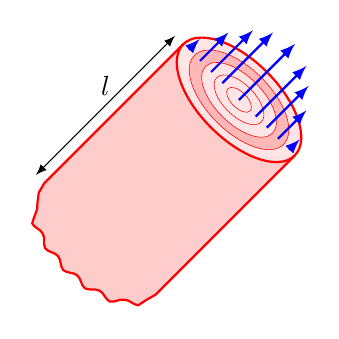
\begin{tikzpicture}[scale=.5, rotate=45]
    \begin{scope}[thick, red, decoration={snake,amplitude=1, pre length=4,post length=4}]
        \filldraw[fill opacity=.1] (0,0) circle[x radius=1, y radius=2];
        \draw (0,2) -- (-5,2) (0,-2) -- (-5,-2) decorate{arc[x radius=1, y radius=2, start angle=270, end angle=90]};
        \fill[opacity=.2] (-5,2) -- (0,2) arc[x radius=1, y radius=2, start angle=90, end angle=270] (0,-2) -- (-5,-2) decorate{arc[x radius=1, y radius=2, start angle=270, end angle=90]};
    \end{scope}
    \foreach \r/\v in {.2,.4,.6,.8}
    {
        \draw[very thin, red] (0,0) circle[x radius=\r, y radius=2*\r];
    }
    \fill[red, opacity=.2, even odd rule] (0,0) circle[x radius=.6, y radius=1.2] circle[x radius=.8, y radius=1.6];
    \foreach \r/\v in {0/1, .3/.91, .5/.75, .7/.51, .9/.19}
    {
        \draw[thick, blue,-latex] (0,2*\r) -- (2*\v,2*\r);
        \draw[thick, blue,-latex] (0,-2*\r) -- (2*\v,-2*\r);
    }
    \draw[latex-latex] (-5,2.3) -- (0,2.3) node[pos=.5, above]{$l$};
\end{tikzpicture}
 
\end{center} 

A cause du frottement contre les parois du tube, la vitesse du sang 
est maximale au centre du vaisseau et est nulle au niveau des parois. 
La vitesse en un point à distance $r$ de l'axe central est donnée (en 
{cm/s}) par
\begin{equation}
v(r)=\frac {P} {4 \eta l} (R^2-r^2) \label{vitesse-sang}
\end{equation}
où $P$ est la différence de pression entre les deux extrémités du tube 
et $\eta$ la viscosité du sang.


\begin{enumerate}\setcounter{enumi}{1}
	\item Calculer le débit à partir de (\ref{debit-sang}) en utilisant 
	l'expression (\ref{vitesse-sang}) de $v(r)$. Cette expression de $F$ 
	est appelée la loi de Poiseuille.
	\item L'hypertension est due au rétrécissement des artères. Pour maintenir 
	le même débit, le coeur doit pomper plus fort, ce qui augmente la pression 
	sanguine. Utiliser la loi de Poiseuille pour montrer que si $R_0$ et $P_0$ 
	sont les valeurs normales du rayon et de la pression, $R$ et $P$ les valeurs 
	lors de l'hypertension, alors conserver le même débit sanguin impliquera la 
	relation
	\begin{equation}
	\frac P {P_0} = \left(\frac {R_0} R\right) ^4.
	\end{equation}
	En déduire que si le rayon de l'artère est réduit aux trois quarts de sa 
	valeur normale, la pression sanguine a plus que triplé.
\end{enumerate}
\finenonce

\indication
Une primitive de $ x^n $ est $ \frac{1}{n+1} x^{n+1} + C $, $ C \in \Rr $.  
\finindication

\correction

\video{oieMpRS-PYg}

\sauteligne
\begin{enumerate} 
	\item 
	Soit $v(r) \equiv v$ constante sur $[0,R]$. Alors la formule (\ref{debit-sang}) 
	implique 
	\begin{equation*} 
		F = \int_0^R 2 \pi r v dr = 2 \pi v \int_0^R r dr 
		= 2 \pi v \left[\frac{r^2}{2}\right]_0^R 
		= \underbrace{\pi R^2}_{\text{\tiny section du vaisseau}} \cdot 
		\underbrace{v}_{\text{\tiny vitesse}}.  
	\end{equation*} 

	\item 
	On a 
	\begin{equation*} 
		F = \int_0^R 2 \pi r \frac {P} {4 \eta l} (R^2-r^2) dr 
		= \frac{\pi P}{2 \eta l} \int_0^R (R^2 r -r^3) dr 
		= \frac{\pi P}{2 \eta l} \left[\frac{R^2 r^2}{2} - \frac{r^4}{4}\right]_0^R 
		= \frac{\pi P}{2 \eta l} \left(\frac{R^4}{2} - \frac{R^4}{4}\right) 
		= \frac{\pi P R^4}{8 \eta l}. 
	\end{equation*} 
	\item 
	On a $ F = \frac{\pi P R^4}{8 \eta l} $ et $ F_0 = \frac{\pi P_0 R_0^4}{8 \eta l} $. 
	Alors $ F = F_0 $ implique 
	\begin{equation*} 
		\frac{\pi P R^4}{8 \eta l} = \frac{\pi P_0 R_0^4}{8 \eta l} 
		\quad \Longleftrightarrow \quad 
		P R^4 = P_0 R_0^4 
		\quad \Longleftrightarrow \quad 
		\frac{P}{P_0} = \left(\frac{R_0}{R}\right)^4. 
	\end{equation*} 
	Si $ R = \frac{3}{4} R_0 $, alors 
	\begin{equation*} 
		P = \left(\frac{4}{3}\right)^4 P_0 > 3 P_0. 
	\end{equation*} 
\end{enumerate} 
\fincorrection
\finexercice


\end{document}